\documentclass[11pt]{article}

\usepackage[margin=1in]{geometry}
\usepackage{amsmath,amssymb,amsfonts}
\usepackage{booktabs}
\usepackage{graphicx}
\usepackage{hyperref}
\usepackage{xcolor}
\usepackage{longtable}
\usepackage{pdflscape}
\usepackage{multirow}
\usepackage[affil-it]{authblk}
\usepackage{tikz}
\usetikzlibrary{arrows.meta, positioning}
\usepackage{lineno}
\usepackage[numbers,sort&compress]{natbib}

\renewcommand{\arraystretch}{1.3}
\emergencystretch=1.5em

\title{\emph{Cis}-pQTL Mendelian Randomization Is Uninformative for Enzyme Inhibitors and Receptor Antagonists:\\A Pre-Registered Evaluation of 195 Phase~III Drug-Target Pairs}

\author{Elliot Tower}
\affil{Independent Researcher \\ \texttt{elliot@elliottower.ai}}
\date{}

\begin{document}
\linenumbers
\maketitle

\begin{abstract}
Null genetic evidence is routinely interpreted as evidence against a drug target. For enzyme inhibitors and receptor antagonists, however, the null reflects what the instrument measures rather than the drug's effect: \emph{cis}-pQTL Mendelian randomization (MR) instruments protein abundance, while most small-molecule drugs act on protein function without changing levels. In a pre-registered evaluation of 195 Phase~III drug-target pairs (138 with available instruments), MR detected only one mechanism class: soluble ligand neutralization (AUC~$= 0.89$, permutation $p < 0.001$; balanced accuracy~$= 0.66$, $n = 22$). All other mechanisms performed at chance. Among approved activity-blocking drugs, 19 of 21 returned null MR, and 100\% had zero GWAS credible set evidence on Open Targets. ACE inhibitors, DPP4 inhibitors, and EGFR inhibitors receive no signal in this evaluation from the genetic evidence channel that pipelines use for target discovery. Annotating genetic evidence with drug mechanism would address this.
\end{abstract}

\noindent\textbf{Keywords:} Mendelian randomization, \emph{cis}-pQTL, drug-target validation, mechanism of action, pipeline bias, genetic evidence

\section{Introduction}
\label{sec:intro}

Drug targets with genetic support have approximately twice the historical Phase~III approval rate \cite{nelson2015support, king2019greater, minikel2024refining, schmidt2020genetic, trajanoska2023target}. Platforms such as Open Targets aggregate genetic evidence---including \emph{cis}-pQTL Mendelian randomization (MR)---into composite scores that guide target prioritization across the pharmaceutical industry \cite{ochoa2021opentargets, trajanoska2025genomics}. A \emph{cis}-pQTL serves as a genetic instrument for circulating protein abundance. For a drug that depletes a circulating target---a biologic neutralizing a soluble cytokine---the pQTL instruments the same quantity the drug perturbs. For a drug that blocks enzymatic activity or antagonizes a receptor, the protein remains at normal circulating levels while its function is inhibited. Gill et al.\ \cite{gill2021mendelian} articulated this mismatch conceptually, and Zheng et al.\ \cite{zheng2023instrumenting} questioned whether pQTL instruments genuinely proxy drug action. We provide a pre-registered empirical test: classifying drug-target pairs into five mechanism categories shows that MR informativeness is concentrated in one of them (soluble ligand neutralization) and absent across the rest.

\begin{figure}[t]
\centering
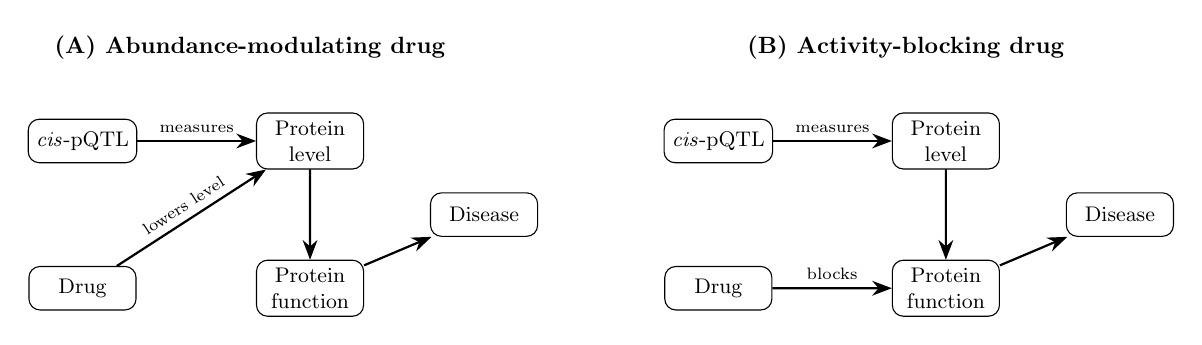
\begin{tikzpicture}[scale=0.85, every node/.style={transform shape},
    every node/.append style={font=\small},
    box/.style={draw, rounded corners, minimum width=1.6cm, minimum height=0.65cm, align=center},
    arr/.style={-{Stealth[length=2.5mm]}, thick},
]

\node[font=\normalsize\bfseries] at (2.5, 1.4) {(A) Abundance-modulating drug};

\node[box] (snpA) at (0, 0) {\emph{cis}-pQTL};
\node[box] (lvlA) at (3.4, 0) {Protein\\level};
\node[box] (funA) at (3.4, -2.2) {Protein\\function};
\node[box] (disA) at (6.0, -1.1) {Disease};
\node[box] (drugA) at (0, -2.2) {Drug};

\draw[arr] (snpA) -- node[above, font=\scriptsize, midway] {measures} (lvlA);
\draw[arr] (lvlA) -- (funA);
\draw[arr] (funA) -- (disA);
\draw[arr] (drugA) -- node[above, font=\scriptsize, midway, sloped] {lowers level} (lvlA);


\begin{scope}[xshift=9.5cm]

\node[font=\normalsize\bfseries] at (2.8, 1.4) {(B) Activity-blocking drug};

\node[box] (snpB) at (0, 0) {\emph{cis}-pQTL};
\node[box] (lvlB) at (3.4, 0) {Protein\\level};
\node[box] (funB) at (3.4, -2.2) {Protein\\function};
\node[box] (disB) at (6.0, -1.1) {Disease};
\node[box] (drugB) at (0, -2.2) {Drug};

\draw[arr] (snpB) -- node[above, font=\scriptsize, midway] {measures} (lvlB);
\draw[arr] (lvlB) -- (funB);
\draw[arr] (funB) -- (disB);
\draw[arr] (drugB) -- node[above, font=\scriptsize, midway, sloped] {blocks} (funB);


\end{scope}

\end{tikzpicture}
\caption{Causal diagrams for \emph{cis}-pQTL Mendelian randomization under two drug mechanisms. (A)~An abundance-modulating drug (such as anti-TNF) reduces circulating protein level, the same node the \emph{cis}-pQTL instruments. The MR estimate is causally aligned with the drug's perturbation. (B)~An activity-blocking drug (such as an ACE inhibitor) inhibits protein function without altering circulating levels. The \emph{cis}-pQTL still instruments protein level, which the drug does not change; larger samples narrow the confidence interval around this null without detecting the drug's effect on protein function.}
\label{fig:dag}
\end{figure}

We predicted that null pQTL-MR for activity-blocking targets would be misinterpreted as ``no genetic support'' when the instrument-target mismatch means the pQTL cannot detect the drug-relevant biology regardless of sample size. We tested this with pre-registered mechanism categories (SHA-256 hashed classifications frozen before outcome adjudication), an Open Targets genetic evidence query, and a pre-selected ACE inhibitor case study (Figure~\ref{fig:dag}).

\section{Results}

\subsection{Approved activity-blocking drugs}
\label{sec:blindspot}

From 211 unique gene--disease pairs at the intersection of pQTL instruments and Open Targets Phase~III targets, 195 were evaluable (63 SUCCESS, 132 FAILURE; base rate 32.3\%). Of these, 138 had at least one \emph{cis}-pQTL instrument available for MR analysis; the remaining 57 lacked instruments, predominantly due to protein assay coverage gaps (missingness characterization in Supplementary~S4). Among approved activity-blocking drugs in the dataset, 19 of 21 with MR results (90.5\%) have null pQTL-MR ($p \geq 0.05$)---including ACE inhibitors, DPP4 inhibitors, EGFR inhibitors, cholinesterase inhibitors, and PARP inhibitors. A standard pQTL-MR screen would deprioritize all of them.

The Open Targets GWAS credible set query provides a partially overlapping but distinct line of evidence: it draws on genome-wide association data from the GWAS Catalog (some of which overlaps with the outcome GWAS consortia used in our MR analysis), so the two analyses are not fully independent. With that caveat, the pattern is consistent: among all 30 approved activity-blocking targets, 100\% have zero GWAS credible set evidence (the genetic association channel used for target discovery), exceeding the pre-registered threshold of $\geq 40\%$. The mean GWAS credible set score for abundance-modulating targets ($0.097$) is $7.8\times$ higher than for activity-blocking targets ($0.012$).

\subsection{MR performance by mechanism subcategory}
\label{sec:gradient}

MR performance is concentrated in a single mechanism subcategory (Table~\ref{tab:gradient}).

\begin{table}[t]
\centering
\caption{MR performance by pre-registered mechanism subcategory (V6). BA~$= 0.658$ for soluble ligand neutralization; all other subcategories cluster near chance.}
\label{tab:gradient}
\small
\begin{tabular}{llcccccccl}
\toprule
& Subcategory & $n$ & TP & FP & Sens & Spec & BA & 90\% CI & AUC \\
\midrule
A1 & Soluble ligand neutralization & 22 & 4 & 1 & 0.400 & 0.917 & 0.658 & $[0.51, 0.80]$ & $0.892^{***}$ \\
A2 & Surface target depletion & 20 & 1 & 2 & 0.143 & 0.846 & 0.495 & $[0.37, 0.64]$ & 0.368 \\
A3 & Indirect abundance & 17 & 0 & 1 & 0.000 & 0.938 & 0.469 & $[0.43, 0.50]$ & ---$^\dagger$ \\
B1 & Enzyme inhibitor & 38 & 2 & 3 & 0.118 & 0.857 & 0.487 & $[0.40, 0.58]$ & 0.476 \\
B2 & Receptor/kinase antagonist & 38 & 0 & 1 & 0.000 & 0.971 & 0.485 & $[0.46, 0.50]$ & 0.588 \\
\bottomrule
\multicolumn{10}{l}{\scriptsize $^{***}$Permutation $p < 0.001$. $^\dagger$1 SUCCESS case; AUC not interpretable; row retained as pre-registered subcategory.} \\
\end{tabular}
\normalsize
\end{table}

Soluble ligand neutralization (A1) is the only subcategory with above-chance MR performance: the threshold-free AUC is $0.892$ (permutation $p < 0.001$), and BA~$= 0.658$ (95\% CI $[0.48, 0.83]$; pre-registered 90\% CI $[0.51, 0.80]$). The four true positives in A1---IL12B$\rightarrow$Crohn's ($p = 8 \times 10^{-26}$), IL12B$\rightarrow$UC ($p = 5 \times 10^{-17}$), IL6R$\rightarrow$RA ($p = 1.5 \times 10^{-9}$), IL6R$\rightarrow$JIA ($p = 0.011$)---are all targets where the drug (ustekinumab, tocilizumab) directly neutralizes the same circulating molecule the pQTL instruments. These four pairs represent two unique genes (IL12B and IL6R), each with two disease indications; the A1 signal should be interpreted as resting on two independent biological targets rather than four independent observations. Gene-deduplicated A1 AUC remains high ($0.878$) but BA drops to $0.571$ ($n = 14$ unique genes), so the A1 result needs replication with additional soluble ligand targets. The fifth abundance-stratum true positive, IFNAR1$\rightarrow$MS ($p = 0.005$), falls in A2 (surface target depletion).

Four of five abundance-stratum true positives (80\%) fall in subcategory A1, compared to the 37\% expected under proportional distribution (pre-registered hypothesis H5.2, confirmed). Sensitivity in A1 (0.400) is 3.2$\times$ higher than in A2+A3 combined. The collapsed three-way and additional hypothesis tests are in Supplementary~S6.

\subsection{Binary stratification}
\label{sec:binary}

The binary mechanism stratification matches the predicted pattern. For activity-blocking targets ($n = 76$), MR is uninformative: BA~$= 0.511$ (95\% CI $[0.447, 0.590]$), AUC~$= 0.526$ (permutation $p = 0.37$), sensitivity~$= 0.095$. The two activity-arm true positives (ALDH5A1$\rightarrow$MDD, $p = 0.041$; IMPA1$\rightarrow$MDD, $p = 0.026$) are consistent with chance: at a 5\% threshold with 21 SUCCESS pairs, approximately one true positive is expected even under the null. For abundance-modulating targets ($n = 59$), MR trends positive: BA~$= 0.590$ (95\% CI $[0.478, 0.709]$); AUC~$= 0.665$ (permutation $p = 0.023$).

\subsection{Case study: ACE inhibitors}
\label{sec:ace}

Angiotensin-converting enzyme (ACE) inhibitors make the domain-of-validity boundary concrete. ACE is a zinc-dependent carboxydipeptidase that converts angiotensin~I to the vasoconstrictor angiotensin~II. ACE inhibitors---ramipril, enalapril, lisinopril---bind the enzyme's active site and block this conversion; the ACE protein itself remains present at normal or elevated circulating levels. A \emph{cis}-pQTL for ACE (rs4344, INTERVAL proteomics) instruments circulating ACE \emph{protein abundance}, a quantity that ACE inhibitors do not perturb. The MR result is null for both indications: chronic kidney disease ($\hat{\beta} = 0.006$, $p = 0.81$) and myocardial infarction ($\hat{\beta} = 0.020$, $p = 0.26$). Both are clinical successes.

The clinical evidence for ACE inhibitors is among the strongest in cardiovascular medicine. The SOLVD trial showed that enalapril reduced all-cause mortality in chronic heart failure \cite{solvd1991}; the HOPE trial showed that ramipril reduced the composite of MI, stroke, or cardiovascular death by 22\% ($p < 0.001$) in high-risk patients \cite{hope2000}; the EUROPA trial reported comparable benefits for perindopril in stable coronary disease \cite{europa2003}. Lisinopril alone receives over 76~million prescriptions per year in the United States \cite{clincalc2023}. A target-validation pipeline that treats a null \emph{cis}-pQTL MR result as evidence against pursuing a target would deprioritize ACE on the basis of an instrument that measures a quantity the drug does not change.

\subsection{Robustness}
\label{sec:robustness}

Leave-one-disease-out analysis yields a BA range of $[0.538, 0.584]$ (SD~$= 0.010$); no single disease drives the result. Gene-level deduplication ($n = 80$ unique genes) yields BA~$= 0.556$, indicating that multi-disease gene duplication does not inflate the composite.

Missingness is non-random: among abundance-modulating pairs, the SUCCESS rate is higher in missing pairs (52.9\%, $n = 34$) than in analyzed pairs (30.5\%, $n = 59$), indicating that the abundance arm's performance may be underestimated (Supplementary~S4). In the activity arm, missingness is favorable (22.7\% SUCCESS among missing vs.\ 27.6\% among analyzed).

The binary threshold ($p < 0.05$) does not drive the result. In threshold sensitivity analysis, the abundance arm shows stable BA across thresholds ($0.57$--$0.61$ for $p < 0.001$ through $p < 0.10$), while the activity arm remains at BA~$= 0.50$ for all thresholds below $p < 0.01$ (Supplementary~S7). Effect direction concordance (based on ChEMBL action types) is 59\% overall ($78/132$) and 67\% among significant pairs ($10/15$), only modestly above the 50\% expected by chance. Among the four A1 true positives, the two IL12B pairs are direction-concordant (positive beta, as expected for an inhibitor), while the two IL6R pairs are discordant---consistent with IL-6 receptor's dual role in classical and \emph{trans}-signaling, where reduced soluble IL6R can increase inflammation. Full robustness analyses are in the online repository.

Three secondary stratifications were pre-specified (Supplementary~S8). Instrument source and sample overlap leave the composite estimate intact: EpiGraphDB- and UKB-PPP-instrumented pairs score $0.640$ and $0.532$ with overlapping intervals, and excluding the five overlap-flagged pairs moves BA from $0.578$ to $0.584$. Disease area does not. Oncology pairs are scored at chance (BA~$= 0.489$ [$0.466$, $0.500$], no true positives) while non-oncology pairs reach $0.595$ [$0.525$, $0.664$], and the intervals do not overlap. Oncology targets in this set are predominantly receptor tyrosine kinases and other activity-blocking mechanisms, so the composite estimate is a mixture that understates the contrast between mechanism classes.

\section{Discussion}
\label{sec:discussion}

Gill et al.\ \cite{gill2021mendelian} predicted that pQTL-MR would perform poorly for activity-blocking targets on conceptual grounds. These data support that prediction and show the split is finer than binary: even within the abundance-modulating stratum, only the soluble ligand subclass (A1) carries detectable signal. MR informativeness tracks the alignment between the drug's mechanism and the pQTL instrument (Figure~\ref{fig:dag}). Surface target depletion (A2), where the pQTL instruments a shed soluble form while the drug acts on the membrane-bound protein, already falls to chance.

The ACE case study makes the mismatch concrete. The pQTL-MR null ($p = 0.81$ for CKD, $p = 0.26$ for MI) is the correct answer to the wrong question: the instrument asks what happens when ACE protein levels decrease, while ACE inhibitors block catalytic activity at unchanged protein levels. This is not resolvable by increasing sample size---larger proteomics cohorts will produce tighter confidence intervals around the same null, because the causal axis the drug acts on (enzymatic function) is orthogonal to the axis the instrument measures (protein level). The same logic applies to every enzyme inhibitor and receptor antagonist in the dataset.

A practical corrective would be to annotate genetic evidence by drug mechanism before scoring. Genetics-guided priority scores such as GPS \cite{duffy2024gps} and direction-of-effect frameworks \cite{chen2025direction} aggregate genetic evidence without conditioning on drug mechanism; a mechanism flag could improve their predictions for the activity-blocking targets that currently receive no signal. Druggable genome pipelines \cite{finan2017druggable} and platforms such as Open Targets could implement this as a simple routing rule: for compounds classified as abundance-modulating, include pQTL-MR evidence in the composite score; for activity-blocking compounds, exclude it or replace it with activity-relevant instruments. Even a binary flag (abundance vs.\ activity) on the evidence channel would separate the targets for which pQTL-MR carries information from those for which it does not.

Alternative genetic instruments could in principle provide evidence for activity-blocking targets. Gain-of-function coding variants, enzyme-activity QTLs, or splice QTLs affecting catalytic domains would probe the causal axis that matters for these drug classes. Expression QTLs (eQTLs) test a distinct hypothesis from pQTLs---whether gene expression changes, rather than protein levels, predict disease---but face a similar limitation for most activity-blocking targets: ACE inhibitors do not alter ACE mRNA expression, and receptor antagonists generally leave receptor transcription unchanged. eQTLs would complement pQTLs primarily for targets where the drug's downstream effect includes transcriptional feedback. Few such activity-specific instruments are currently available at genome-wide scale, but targeted characterization for high-priority drug classes would be feasible.

\paragraph{Limitations.}
The abundance arm is underpowered. At $n = 22$, power to detect a true BA of $0.66$ is approximately 42\%; $n \approx 55$ A1 pairs would be needed for 80\% power, and $n \approx 150$ for a more conservative true BA of $0.60$. The 90\% CI lower bound for A1 ($0.51$) barely excludes $0.50$, and the 95\% CI ($[0.48, 0.83]$) includes it. The threshold-free AUC ($0.892$, permutation $p < 0.001$) provides stronger evidence of discriminative ability, but confirmation with larger samples is needed.

Cross-platform concordance of the instruments is untested. The two \emph{cis}-pQTL catalogs contribute disjoint proteins, so no protein is instrumented on both SomaScan and Olink and no within-protein comparison of platform-specific effect estimates is possible in this dataset. Analyses pooling assay technologies should establish this separately.

All MR estimates use single-SNP Wald ratios. Multi-instrument \emph{cis}-MR (restricting to the \emph{cis} region to minimize horizontal pleiotropy) could increase power, and the present findings should be confirmed under that design. Single-SNP Wald ratios are subject to winner's curse, biasing toward the null---a conservative direction for the activity arm but one that could mask signal in the abundance arm.

Mechanism classifications were assigned by a single rater. Pre-registration mitigates outcome-dependent classification, but not misclassification error. As a protein-class consistency check, all 66 genes in subcategories A1, A2, B1, and B2 were verified against UniProt/HGNC annotations: every B1 gene encodes an enzyme, every B2 gene a receptor or kinase, every A1 gene a soluble protein, and every A2 gene a membrane-bound surface protein. The labels therefore match the target's molecular class, though this check does not independently validate the drug-level mechanism call (e.g., whether a given drug acts by depleting vs.\ blocking its target). To test whether plausible reclassifications could change the result, we identified 16 borderline pairs (11 genes) at the abundance/activity boundary---primarily MMP inhibitors (A3, arguably B1) and integrin antagonists (A2, arguably B2)---and swapped all of them simultaneously. Activity-arm BA changed from $0.511$ to $0.505$ ($\Delta = -0.006$); A1 AUC ($0.892$) was invariant because no A1 genes are borderline. The result holds under the reclassifications we could identify, though a second rater would be a stronger check. The frozen gene-to-subcategory assignments are publicly available for independent replication.

Loss-of-function burden tests from Genebass \cite{karczewski2022genebass} returned null results (AUC~$= 0.538$, $p = 0.49$), indistinguishable from chance at 450k exomes. Only 7 of 132 pairs reached nominal significance under the LoF burden test, reflecting insufficient carrier counts (${\sim}10$--$100$ pLoF carriers per gene). Testing the mechanism dissociation with orthogonal functional instruments requires larger exome cohorts anticipated by gnomAD~v5 and All of Us.

\emph{Cis}-pQTL MR primarily detects soluble ligand targets and is uninformative for activity-blocking drug classes in this dataset. Genetic evidence screens that do not condition on drug mechanism risk systematically deprioritizing activity-blocking targets on the basis of an instrument that measures a quantity these drugs do not change.

\section{Methods}
\label{sec:methods}

\subsection{Data sources}

Genetic instruments were drawn from two sources: the published EpiGraphDB \emph{cis}-pQTL MR catalog \cite{zheng2020phenome}, based on the INTERVAL study \cite{sun2018interval} (${\sim}1{,}740$ proteins, $N \approx 3{,}300$, SomaScan), and UK Biobank Pharma Proteomics Project (UKB-PPP) \emph{cis}-pQTLs \cite{sun2023ukbppp} (${\sim}2{,}900$ proteins, $N \approx 54{,}000$, Olink). Each protein used one instrument: the sentinel \emph{cis}-pQTL (lowest $p$ among conditionally independent \emph{cis} signals as reported by the source study). Multi-SNP IVW \cite{burgess2013ivw} and \emph{trans}-pQTL results were excluded a priori because of their vulnerability to horizontal pleiotropy. Drug targets were taken from the Open Targets Platform \cite{ochoa2021opentargets}, from which all compounds reaching Phase~III were retrieved and linked to their mechanistic gene targets algorithmically.

For each disease, a non-UKB outcome GWAS was selected to avoid sample overlap with UKB-PPP instruments. Sources included FinnGen R10 \cite{kurki2023finngen}, CARDIoGRAMplusC4D, IMSGC, PGC, IIBDGC, ILCCO/TRICL, and disease-specific consortia (full mapping in Supplementary~S3). MR estimates were single-SNP Wald ratios: $\hat{\beta} = \beta_{\text{outcome}} / \beta_{\text{exposure}}$, $\text{SE} = |\text{SE}_{\text{outcome}} / \beta_{\text{exposure}}|$. \emph{Cis}-pQTLs from UKB-PPP ($N \approx 54{,}000$) typically have $F > 100$; winner's curse from discovery-sample inflation \cite{burgess2011weak} biases MR estimates toward the null---a conservative direction.

All mechanism classifications and hypotheses were frozen (SHA-256 hashed) before outcome adjudication (protocol versioning and deviation log in Supplementary~S1). Outcome labels were adjudicated independently against FDA/EMA records and ClinicalTrials.gov: SUCCESS denotes regulatory approval or a met Phase~III primary endpoint; FAILURE denotes a failed primary endpoint or discontinuation.

\subsection{Mechanism classification}

Each pair was classified by drug mechanism into \emph{abundance-modulating} (the drug reduces circulating protein level, matching the pQTL perturbation), \emph{activity-blocking} (the drug inhibits enzymatic activity or blocks a receptor without changing the target protein's measured circulating level), or \emph{mixed} (both mechanisms apply). Classification was determined by the drug's pharmacological action, not the MR result. To test whether MR informativeness follows a gradient, the binary classification was refined into five subcategories ordered by predicted alignment between the drug mechanism and the pQTL instrument: A1, soluble ligand neutralization ($n = 22$; drug directly binds or neutralizes the same circulating protein the pQTL instruments); A2, surface target depletion ($n = 20$; drug targets a cell-surface protein, pQTL instruments the shed soluble form); A3, indirect abundance modulation ($n = 17$; drug modulates protein levels indirectly); B1, enzyme inhibitor ($n = 38$; drug blocks the enzymatic active site, protein present at normal levels); and B2, receptor/kinase antagonist ($n = 38$; drug blocks receptor or kinase signaling). Gene-to-subcategory assignments were frozen before analysis. A collapsed three-way grouping combines A1+A2 as \emph{direct neutralization}, A3 as \emph{indirect abundance}, and B1+B2 as \emph{function blocking}.

For each gene-disease pair, we queried the Open Targets Platform GraphQL API for the overall association score and the GWAS credible set evidence score. The pre-registered prediction was that $\geq 40\%$ of approved activity-blocking targets would have zero GWAS credible set evidence.

\subsection{Statistical analysis}

The classifier carries zero free parameters: MR $p < 0.05 \rightarrow$ predict SUCCESS; MR $p \geq 0.05 \rightarrow$ predict FAILURE. The threshold $p < 0.05$ is the field-standard MR significance criterion and was not optimized on these data. Balanced accuracy (BA) with 10{,}000-iteration bootstrap 95\% CI was computed for each subcategory and for the binary strata; the pre-registered falsification criterion used a 90\% CI (CI lower bound $> 0.50$). AUC was computed using the Wilcoxon--Mann--Whitney $U$-statistic with $-\log_{10}(p)$ as the continuous score, with significance assessed by 10{,}000-iteration permutation test. All hypotheses and decision rules were pre-declared before adjudication. No correction for multiple comparisons was applied across the five subcategories because each hypothesis was pre-registered and directional; the A1 permutation $p < 0.001$ survives Bonferroni correction across all five tests ($\alpha_{\text{adj}} = 0.01$).

\section*{Data Availability}

All data are available at \url{https://github.com/elliottower/pqtl-mr-domain-of-validity}. The repository contains the full per-pair classification table, all six pre-registration protocol versions (V1--V6) with SHA-256 hashes and the deviation log, the mechanism subcategory assignments, and Open Targets query results. A DOI-versioned snapshot is archived on Zenodo (\url{https://zenodo.org/records/21207429}). This study uses only publicly available summary-level data.

\section*{Code Availability}

All analysis scripts are available at the repository listed under Data Availability, under the MIT License.

\section*{Declarations}

\paragraph{Ethics approval and consent to participate.}
This study uses exclusively publicly available, summary-level genetic association data. No individual-level data, human subjects, or animal subjects were involved. No ethical approval was required.

\paragraph{Competing interests.}
The author declares no competing interests.

\paragraph{Funding.}
None. This work was conducted independently.

\paragraph{Authors' contributions.}
E.T. conceived the study, designed and pre-registered the protocol, collected and adjudicated data, performed all analyses, and wrote the manuscript.

\paragraph{Acknowledgements.}
AI tools (Claude Code, Perplexity Pro) were used for code drafting and manuscript drafting. All experimental design and conclusions are the author's.

\begin{thebibliography}{99}

\bibitem{gill2021mendelian}
Gill, D., Georgakis, M.K., Walker, V.M., Schmidt, A.F., Gkatzionis, A., et al.
\newblock Mendelian randomization for studying the effects of perturbing drug targets.
\newblock \emph{Wellcome Open Research}, 6:16, 2021.

\bibitem{king2019greater}
King, E.A., Davis, J.W., and Degner, J.F.
\newblock Are drug targets with genetic support twice as likely to be approved?
\newblock \emph{PLoS Genetics}, 15(12):e1008489, 2019.

\bibitem{minikel2024refining}
Minikel, E.V. et al.
\newblock Refining the impact of genetic evidence on clinical success.
\newblock \emph{Nature}, 629(8012):624--629, 2024.

\bibitem{nelson2015support}
Nelson, M.R. et al.
\newblock The support of human genetic evidence for approved drug indications.
\newblock \emph{Nature Genetics}, 47(8):856--860, 2015.

\bibitem{ochoa2021opentargets}
Ochoa, D. et al.
\newblock Open Targets Platform: supporting systematic drug-target identification and prioritisation.
\newblock \emph{Nucleic Acids Research}, 49(D1):D1302--D1310, 2021.

\bibitem{zheng2020phenome}
Zheng, J. et al.
\newblock Phenome-wide Mendelian randomization mapping the influence of the plasma proteome on complex diseases.
\newblock \emph{Nature Genetics}, 52(10):1122--1131, 2020.

\bibitem{karczewski2022genebass}
Karczewski, K.J. et al.
\newblock Systematic single-variant and gene-based association testing of thousands of phenotypes in 394,841 UK Biobank exomes.
\newblock \emph{Cell Genomics}, 2(9):100168, 2022.

\bibitem{burgess2013ivw}
Burgess, S., Butterworth, A., and Thompson, S.G.
\newblock Mendelian randomization analysis with multiple genetic variants using summarized data.
\newblock \emph{Genetic Epidemiology}, 37(7):658--665, 2013.

\bibitem{finan2017druggable}
Finan, C. et al.
\newblock The druggable genome and support for target identification and validation in drug development.
\newblock \emph{Science Translational Medicine}, 9(383):eaag1166, 2017.

\bibitem{burgess2011weak}
Burgess, S. and Thompson, S.G.
\newblock Avoiding bias from weak instruments in Mendelian randomization studies.
\newblock \emph{International Journal of Epidemiology}, 40(3):755--764, 2011.

\bibitem{sun2018interval}
Sun, B.B. et al.
\newblock Genomic atlas of the human plasma proteome.
\newblock \emph{Nature}, 558(7708):73--79, 2018.

\bibitem{sun2023ukbppp}
Sun, B.B. et al.
\newblock Plasma proteomic associations with genetics and health in the UK Biobank.
\newblock \emph{Nature}, 622(7982):329--338, 2023.

\bibitem{kurki2023finngen}
Kurki, M.I. et al.
\newblock FinnGen provides genetic insights from a well-phenotyped isolated population.
\newblock \emph{Nature}, 613(7944):508--518, 2023.

\bibitem{solvd1991}
The SOLVD Investigators.
\newblock Effect of enalapril on survival in patients with reduced left ventricular ejection fractions and congestive heart failure.
\newblock \emph{New England Journal of Medicine}, 325(5):293--302, 1991.

\bibitem{hope2000}
The Heart Outcomes Prevention Evaluation Study Investigators.
\newblock Effects of an angiotensin-converting-enzyme inhibitor, ramipril, on cardiovascular events in high-risk patients.
\newblock \emph{New England Journal of Medicine}, 342(3):145--153, 2000.

\bibitem{europa2003}
The EUROPA Investigators.
\newblock Efficacy of perindopril in reduction of cardiovascular events among patients with stable coronary artery disease.
\newblock \emph{Lancet}, 362(9386):782--788, 2003.

\bibitem{clincalc2023}
ClinCalc DrugStats Database.
\newblock Lisinopril drug usage statistics, United States, 2014--2023.
\newblock \url{https://clincalc.com/DrugStats/Drugs/Lisinopril}.

\bibitem{schmidt2020genetic}
Schmidt, A.F. et al.
\newblock Genetic drug target validation using Mendelian randomisation.
\newblock \emph{Nature Communications}, 11:3255, 2020.

\bibitem{trajanoska2023target}
Trajanoska, K. et al.
\newblock From target discovery to clinical drug development with human genetics.
\newblock \emph{Nature}, 620(7975):737--745, 2023.

\bibitem{trajanoska2025genomics}
Trajanoska, K. et al.
\newblock Genomics of drug target prioritization for complex diseases.
\newblock \emph{Nature Reviews Genetics}, 2025.

\bibitem{zheng2023instrumenting}
Zheng, J., Holmes, M.V. et al.
\newblock Drug target Mendelian randomisation: are we really instrumenting drug use?
\newblock \emph{Diabetologia}, 66(7):1156--1161, 2023.

\bibitem{duffy2024gps}
Duffy, \'{A}. et al.
\newblock A human genetics-guided priority score for 19,365 genes and 399 drug indications.
\newblock \emph{Nature Genetics}, 56(1):51--59, 2024.

\bibitem{chen2025direction}
Chen, J., Duffy, \'{A}. et al.
\newblock Genetic evidence informs the direction of therapeutic modulation in drug development.
\newblock \emph{npj Drug Discovery}, 2:24, 2025.

\end{thebibliography}

\end{document}
